\section{The Spatial Compiler}
\label{compiler}

The Spatial compiler provides source-to-source translations from applications in the Spatial language to synthesizable hardware descriptions in Chisel RTL~\cite{chisel}. 
In this section, we describe the compiler's intermediate representation and its key passes, as summarized in Figure~\ref{fig:compilerflow}.
Apart from chisel generation, these passes are common to targeting both FPGAs and the Plasticine CGRA. Details of targeting Plasticine are discussed in prior work~\cite{plasticine}.

%For acceleratable code targeted to FPGAs, the output of the compiler is Chisel code \cite{chisel}, roughly the same level of abstraction as Verilog and VHDL.
%The output for CGRAs depends on the requirements of the hardware target, while host (CPU) code is currently generated in C++.
% Spatial is designed to capture algorithms that are intended to run on reconfigurable architectures,
% which gives rise to analyses and optimizations that are not used in software compilers.
% However, information about the target architecture is important to selectively perform a few extra 
% compiler passes and generate the best code for each.  Currently, Spatial can successfully target both FPGAs and a 
% CGRA, Plasticine, and needs to do certain specializations for each with awareness to what the underlying architecture
% looks like.  Here we will briefly discuss what kinds of specializations are done for the two working targets and how the compiler facilitates these passes.


\begin{figure}
%%% trim = left, bottom, right, top
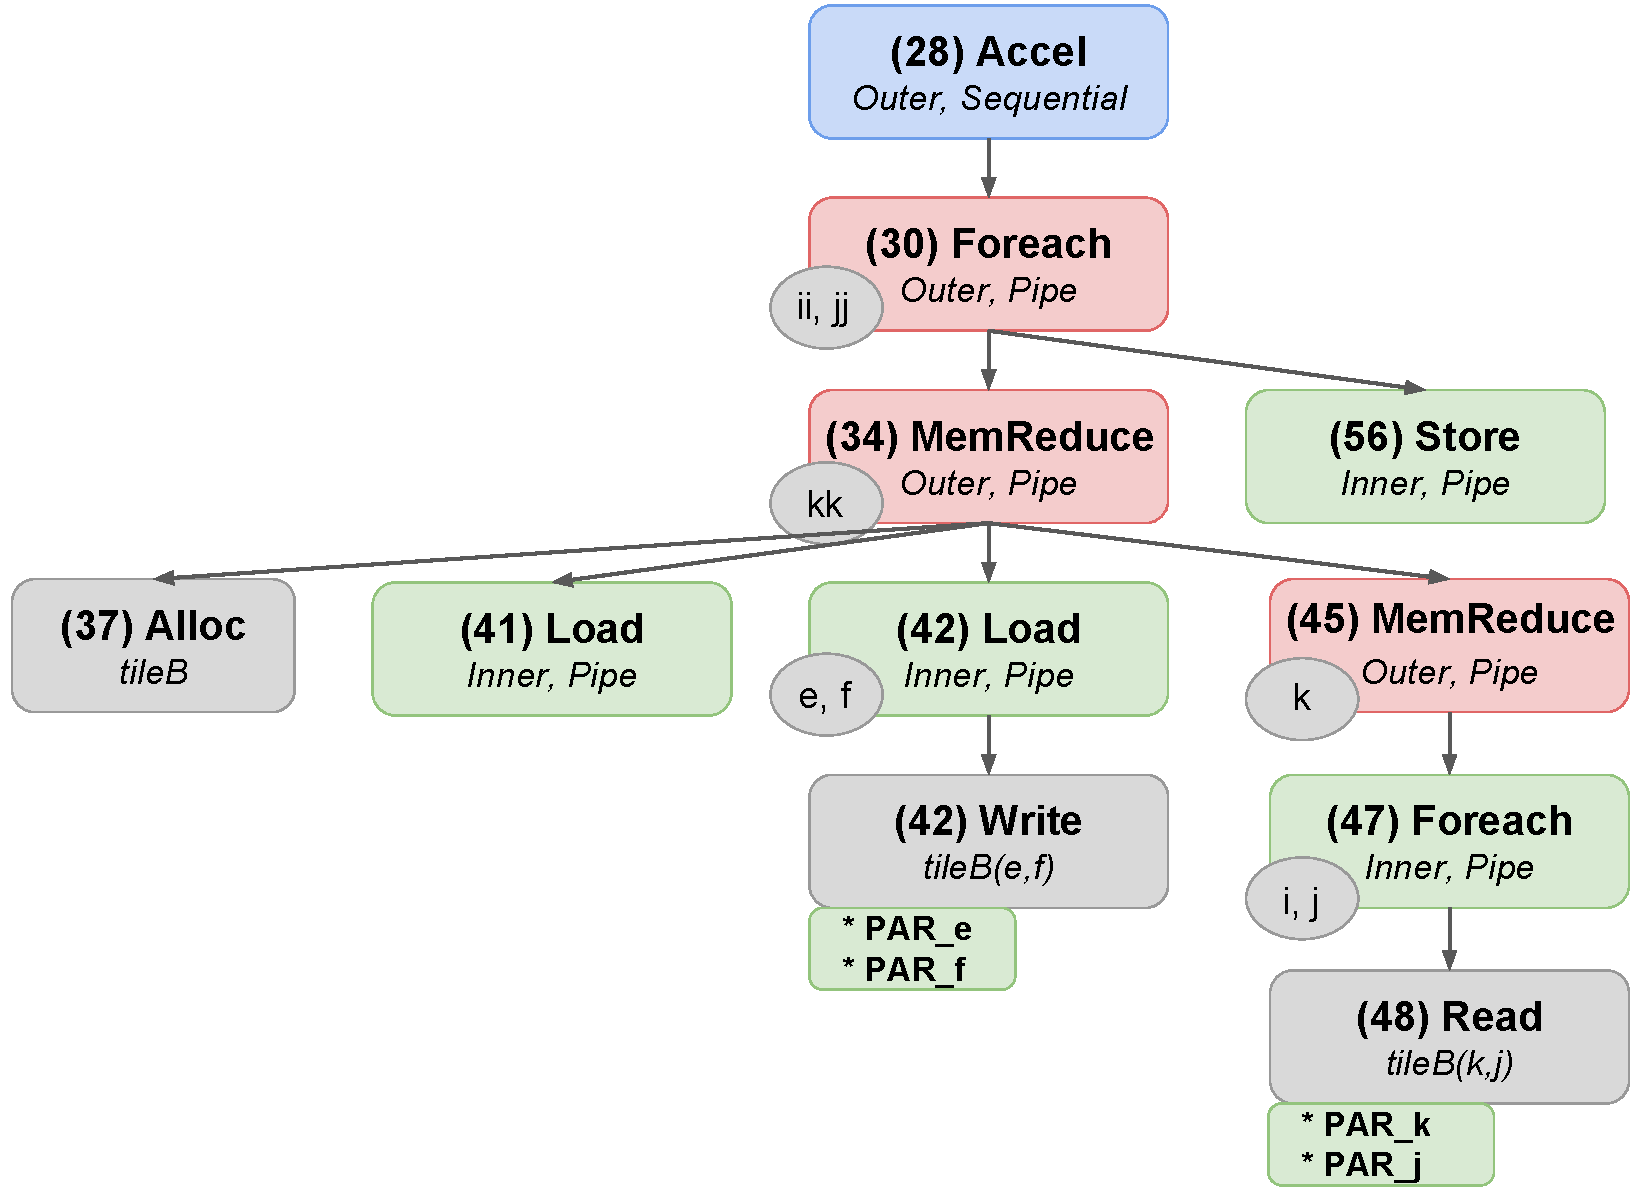
\includegraphics[clip, width=0.9\columnwidth]{figs/control_tree_gemm.pdf}
\vspace{-10pt}
\caption{The control/access tree for the \texttt{\small{SRAM tileB}} in the matrix multiply example in Figure~\ref{fig:matmult}. 
%Control nodes are annotated with their level (outer versus inner), schedule, and loop iterator name. Memory access nodes are annotated with their parallelization factor.
\vspace{-5pt} 
}
\label{fig:controlTree}
\end{figure}

\subsection{Intermediate Representation}

Spatial programs are internally represented in the compiler as a hierarchical dataflow graph (DFG).
Nodes in this graph represent control structures, data operations, and memory allocations, while edges represent data and effect dependencies.
Nesting of controllers directly translates to the hierarchy in the intermediate representation.
Design parameters are kept as graph metadata, such that they can be independently updated without changing the graph itself. 


When discussing DFG transformations and optimizations, it is often useful to think about the graph as a controller/access tree. Figure~\ref{fig:controlTree} shows an example of one such controller tree for the memory {\texttt{\small{tileB}} in the Spatial code example in Figure~\ref{fig:matmult}. Note that transfers between on-chip and off-chip memory expand to a control node which linearly accesses the on-chip memory, in this case by iterators \texttt{e} and \texttt{f}. 
This tree abstracts away most primitive operations, leaving only relevant controller hierarchy and the memory
accesses for a specific memory.


Within the acceleratable subset of Spatial, nodes are formally separated into three categories: 
control nodes, memory allocation nodes, and primitive nodes. 
Control nodes represent state machine structures like \texttt{\small{Foreach}} and \texttt{\small{Reduce}} described in Section~\ref{controls}.
Primitive nodes are operations which may consume, but never produce, control signals, including on-chip memory accesses.
Primitive nodes are further broken down into ``physical'' operations requiring resources and ``ephemeral'' operations which are only used for bookkeeping purposes in the compiler. For example, bit selects and grouping of words into structs require no hardware resources but are used to track necessary wires in the generated code.



% Edit gemm figure here https://docs.google.com/presentation/d/1mScE_E_D2OchZk3xhXiiFQegldOv9iOjSMSic8MITxg/edit?usp=sharing


% The nodes that compose the IR of Spatial provide the handles necessary to do a range of
% hardware optimizations that are specific to spatial architectures.  The combination of
% metadata associated with each node and the hierarchical structure AST that exposes relationships
% between primitives and control structures make it easy to do optimizations on the scheduling of 
% controllers, buffering, banking, and duplication of memory elements, and comprehensive DSE over
% the provided parameter space with low latency.
% \subsection{DRAM Request Consolidation}
% In memory-bound applications, the only way to improve performance is to make better use
% of the available bandwidth.  It is well known that memory bandwidth asymptotically approaches the DRAM's peak bandwidth \todo{is this true?} 
% as the size of each request increases.  This is because of how DRAM pays a penalty for activating and retiring 
% lines of memory cells, and can return more data quickly when consecutive bursts are requested with the same command.

% Unfortunately, there are many applications where the programmer may opt to create logical tensors with 
% relatively small leading dimensions and attempt to load multi-dimensional portions of the structure into on-chip SRAM
% without awareness of how this may thrash the DRAM's controllers in an inefficient way.  For example,
% the programmer may want to solve a multi-objective gradient descent problem that has many training points and very
% few objectives, hence creating a tall and skinny Y matrix.  

% The compiler is able to recognize when the application will be sending out multiple requests to DRAM with
% consecutive addresses, and rewrite the controller to consolidate these into fewer, longer burst commands.
% This means that the user will get fully optimized DRAM requests and physical hardware without needing
% to rethink or change the semantics of the source code. 

\subsection{Control Insertion}

To simplify reasoning about control signals, Spatial requires that control nodes do not contain both physical primitive nodes and other control nodes. The exception to this rule is conditional \texttt{\small{if}} statements, which can be used in the same scope as primitives as long as they contain no control nodes but conditionals themselves.
This requirement is satisfied by a DFG transformation which inserts \texttt{\small{DummyPipe}} control nodes around primitive logic in control bodies which also contain control nodes. The \texttt{\small{DummyPipe}} node is a bookkeeping control structure which is logically equivalent to a loop with exactly one iteration. 
Thereafter, control nodes with primitive nodes are called ``inner'' control nodes, while controllers which contain other nested controllers are called ``outer'' nodes.

% For example, Figure~\ref{fig:matmult} contains some of these nodes. The Foreach in line 32 is an ``outer'' controller, which contains a memory allocation node for tileC 
% (line 33) and another control node, \texttt{\small{MemReduce}} in line 38.  The \texttt{\small{Foreach}} in line 51 is an ``inner'' controller, as it contains
% only primitive nodes generated by the SRAM reads, multiplication, and SRAM store inlined on line 52.


\subsection{Controller Scheduling}
\label{scheduling}
After controller insertion, the compiler will then schedule the operations within each controller.
By default, the compiler will always attempt to pipeline loops regardless of nesting level. 
The behavior of the compiler's scheduler can be overridden by the user using the directives listed in Table~\ref{t:syntaxTable}b.

Inner pipeline schedules are based on their initiation interval. 
The compiler first collects resource initiation intervals for each primitive node in the given controller based on an internal, target-dependent lookup table.
Most primitive operations are pipelined for a resource initiation interval of 1. 
The compiler then calculates all loop carried dependencies within the pipeline based on the dataflow graph.
For non-addressable memories, the total initiation interval is the maximum of path lengths between all dependent reads and the writes. 
For addressable memories, the path length of loop carried dependencies is also multiplied by the difference in write and read addresses.  
If the addresses are loop-independent, the initiation interval is the path length if they may be equal, and 1 if they are provably not equal. If the distance between the addresses cannot be determined statically, the initiation interval is infinite, meaning the loop must be run sequentially.
The total initiation interval is defined as the maximum of the initiation intervals of all loop carried dependencies and all resource initiation intervals. 

The compiler also attempts to pipeline the bodies of outer control nodes in a similar manner, but computes dataflow scheduling in terms of inner control nodes and number of stages rather than primitive nodes and cycles. For example, the outer \texttt{\small{MemReduce}} in line 34 of Figure~\ref{fig:matmult} contains 4 sub-controllers: the load into \texttt{\small{tileA}} (line 41), the load into \texttt{\small{tileB}} (42), the inner \texttt{\small{MemReduce}} (45), and an reduction stage combining intermediate tiles (53). Based on data dependencies, the compiler infers that the two loads can be run in parallel, followed by the inner \texttt{\small{MemReduce}} and the tile reduction. It will also determine that multiple iterations of this outer loop can also be pipelined through these stages.

\subsection{Memory Analysis}
\label{memopts}

Loop parallelization only serves to improve performance if there is sufficient on-chip bandwidth to feed the duplicated computation.
Spatial's memory analysis banks and buffers on-chip memories to maximize this available on-chip read and write bandwidth. 
Memory banking, also called data partitioning, is the process of dividing a memory's address space across multiple physical instances in order to create
additional ports for concurrent accesses within the same controller.
Partitioning is possible when the access patterns are statically predictable and guaranteed to never conflict access the same port/bank. 
While a single port can be time multiplexed, this entirely negates the benefits of parallelization by increasing the whole pipeline's required initiation interval.
Note that while banking can trivially be achieved by memory duplication, Spatial aims to also minimize the total amount of memory resources.  

Spatial leverages the memory partitioning strategy based on conflict polytope emptiness testing described by Wang et. al.~\cite{Wang_banking}. We extend this strategy by accounting for random access patterns and memory accesses across nested loops. Random accesses are modeled as additional dimensions in the conflict polytope as if they were additional loop iterators. Spatial minimizes the number of random access symbols used in this way by identifying affine combinations of random values. For example, an access to a memory at address $x$ and $x+1$ only requires one random variable, $x$, as the second is a predictable, affine function of the first.
Spatial also supports banking per dimension to account for cases where only some dimensions are accessed predictably.

Non-addressed memories like \texttt{\small{FIFOs}} and \texttt{\small{FILOs}} are modeled as addressed memories.
Each access to these memory types is represented as a linear access of all loop iterators around the memory access relative to the memory's definition. Spatial forbids parallelization of outer loops around non-addressed accesses, as this violates the guarantee of equivalent behavior to sequential execution. 

To handle multiple pipelined accesses across stages within an outer loop, Spatial also automatically buffers on-chip memories.
Buffering creates multiple copies of the 
same memory for maintaining versions of the data across overlapped loop iterations. 
Without this optimization, pipeline parallel accesses to the same memory across different stages of a coarse-grain pipeline would not be able to run concurrently.
See Appendix~\ref{banking-appendix} for details on how both banking and buffering are computed.


For example, as shown in Figure~\ref{fig:controlTree}, \texttt{\small{tileB}} has two parallelized accesses, the load on line 42 and the read on line 48. If all (implicit and explicit) parallelization factors are set to 2, this corresponds to 4 accesses per loop. Spatial then builds the access polytope corresponding to all accesses in each loop, and determines the banking strategy that works for both loops. In this example, this means the SRAM will be banked such that each element within a 2x2 square will reside
in a different physical bank to allow fully parallel access. If the \texttt{\small{MemReduce}} on line 34 is pipelined, \texttt{\small{tileB}} will be double buffered to protect the reads (line 48) in one iteration of the outer loop
from the writes (line 42) in the next iteration.


\subsection{Area and Runtime Estimation}
\label{estimate}
Spatial evaluates a given set of parameters by running a pair of estimation passes to approximate the area and runtime  of the application.
These passes are driven by analytical resource and runtime models similar to those used in our prior work on the Delite Hardware Definition Language (DHDL)~\cite{dhdl}, but Spatial expands this approach to account for streaming throughput, arbitrary control flow, and finite state machines. Both runtime and area utilization models are built from a set of about 2000 one-time characterization runs on each target platform.



\subsection{Design Space Exploration}
\label{dse}
The scheduling and memory banking options identified by the compiler, together with loop parallelization and tile size parameters, forms a design space for the application. 
The design tuning pass is an optional compiler pass which allows for fast exploration of this design space in order to make area/runtime design tradeoffs.
When design tuning is enabled, it repeatedly picks design points and evaluates them by rerunning the control scheduling, memory analysis, and estimation analysis passes. The output from this search is a single set of parameters from the Pareto frontier.


%By exposing parameters to the compiler it is possible to automatically perform
%design space exploration on the source code. 
%The code generated will result optimized for speed and logic utilization. 
Unfortunately, application design spaces tend to be extremely large, and exhaustive search on an entire space is often infeasible. Of the benchmarks discussed in Section~\ref{evaluation}, 
only BlackScholes has a relatively small space of about $80,000$ points. While this space can be explored exhaustively by Spatial in a few minutes, other spaces are much larger, spanning $10^6$ to $10^{10}$ points and
taking hours or days to exhaustively search. For example, even with the few explicit design parameters exposed in the code in Figure~\ref{fig:matmult}, when combined with implicit pipelining and parallelization parameters, this code already has about $2.6\times10^8$ potential designs.
DHDL~\cite{dhdl} employed random search after heuristic pruning, reducing the total space by two to three orders of magnitude. However, this approach has high variance on larger design spaces and may inadvertently prune desirable points.

To reduce the variance on larger design spaces, Spatial's design space exploration flow integrates an active learning-based autotuner called HyperMapper~\cite{Bodin2016:PACT16,NardiBSVDK17,Saeedi_ICRA_2017}.
HyperMapper is a multi-objective derivative-free optimizer (DFO), and has already been demonstrated on the SLAMBench benchmarking framework \cite{nardi2015introducing}. 
HyperMapper creates a surrogate model using a Random Forest regressor, and predicts the performance over the parameter space. This regressor is initially built using only few hundred random design point samples and is iteratively refined in subsequent active learning steps.


\subsection{Unrolling}
Following selection of values for design parameters, Spatial finalizes these parameters in a single graph transformation which unrolls loops and duplicates memories as determined by prior analysis passes. 
\texttt{Reduce} and \texttt{MemReduce} patterns are also lowered into their imperative implementations, with hardware reduction trees instantiated from the given reduction function. 
The two \texttt{MemReduce} loops in Figure~\ref{fig:matmult}, for example, will each be lowered into unrolled \texttt{Foreach} loops with explicitly banked memory accesses and explicitly duplicated multiply operations. The corresponding reduction across tiles (lines 52~--~53) are lowered into a second stage of the \texttt{Foreach} with explicit reduction trees matching the loop parallelization. 

\subsection{Retiming}
After unrolling, the compiler retimes each inner pipeline to make sure data and control signals properly line up and ensure that the target clock frequency can be met.
To do this, the compiler orders primitive operations within each pipeline based on effect and dataflow order.
This ordering is calculated using a reverse depth first search along data and effect dependencies. 
A second forward depth first search is then used to minimize delays in reduction cycles.
Based on this ordering, the compiler then inserts pipeline and delay line registers based on lookup tables which map each primitive node to an associated latency. Dependent nodes which have less than a full cycle of delay are kept as combinational operations, with a register only being inserted after the last operation.
This register insertion maximizes the achievable clock frequency for this controller while also minimizing the required initiation interval.



\begin{table*}
\caption{Number of lines of code (LOC), area utilization, and runtime comparisons between SDAccel and Spatial on a single VU9P FPGA. 
For reference, the first row lists the total number of FPGA resources available. LOC improvements are percent improvements from SDAccel. The remaining improvement factors are calculated as $(SDAccel / Spatial)$. 
\vspace{-10pt}
}
\label{t:hls_comp}

\fontsize{8.5}{9.5}\selectfont
\begin{tabular}{llll d{3.0} d{6.0} d{4.0} d{4.0} d{4.1} }
\ml{}                                                           & \ml{}           &\ml{}          & \ml{}                & \mc{LOC}    & \mc{LUTs}         & \mc{BRAM}         & \mc{DSPs}         & \mc{Time (ms)} \\ \toprule
\ml{Benchmark}                                                  & \ml{Data Sizes} &\ml{DSE size}  & \ml{\emph{Capacity}} & \mc{---}    & 914400            & 1680              & 5640              & \mc{---} \\
\midrule

% \multirow{3}{*}{
% \hspace{-8pt}\begin{tabular}{l}
% \bf{AES} \\
% Encryption \\
% \end{tabular}
% }                                                               &
% \multirow{3}{*}{32kB data }
%                                                                 & SDAccel         & 333                  & 338305      & 589               & 0                 & 2.23 \\
%                                                                 &                 & Spatial              & 150         & 600027            & 442               & 9                 & 14.45 \\
%                                                                 &                 & \ml{Relative}        & \mc{54.8\%} & \mc{0.56$\times$} & \mc{1.33$\times$} & \mc{1.33$\times$} & \mc{0.15$\times$} \\ \midrule

\multirow{3}{*}{
\hspace{-8pt}\begin{tabular}{l}
\bf{BS} \\
Black-Scholes \\
Option pricing \\
\end{tabular}
}                                                               &
\multirow{3}{*}{ 960,000 options } 
& \multirow{3}{*}{ $7.7\times 10^4$ }
                                                                & SDAccel         & 175   & 363368      & 550  & 290 & 6.18 \\
                                              &&                & Spatial         & 93    & 698885      & 493  & 945 & 3.79 \\
                                              &                 &                 & \ml{Improvement} & \mc{46.8\%} & \mc{0.52$\times$} & \mc{1.12$\times$} & \mc{0.31$\times$} & \mc{1.63$\times$} \\ \midrule

\multirow{3}{*}{
\hspace{-8pt}\begin{tabular}{l}
\bf{GDA} \\
Gaussian discriminant \\
analysis \\
\end{tabular}
}                                                               &
\multirow{3}{*}{
\hspace{-8pt}\begin{tabular}{l}
1024 rows \\
96 dimensions \\
\end{tabular}
} & \multirow{3}{*}{ $3.0\times 10^{10}$ }
                                                                & SDAccel          & 73    & 356857      & 594   & 108   & 10.75 \\
                                              &&                 & Spatial          & 64    & 378130      & 858   & 216   & 1.27  \\
                                              &&                 & \ml{Improvement} & \mc{12.3\%} & \mc{0.94$\times$} & \mc{0.69$\times$} & \mc{0.50$\times$} & \mc{8.48$\times$} \\ \midrule


\multirow{3}{*}{
\hspace{-8pt}\begin{tabular}{l}
\bf{GEMM} \\
Matrix multiply \\
\end{tabular}
}                                                               &
\multirow{3}{*}{
\hspace{-8pt}\begin{tabular}{l}
A: 1024$\times$1024 \\
B: 1024$\times$1024 \\
\end{tabular}
} 
& \multirow{3}{*}{ $2.6\times 10^8$ }
                                                                & SDAccel          & 110         & 341894            & 674               & 206                & 1207.26 \\
                                              &&                 & Spatial          & 44          & 426295            & 500               & 798               & 878.45 \\
                                              &&                 & \ml{Improvement} & \mc{60.0\%} & \mc{0.80$\times$} & \mc{1.35$\times$} & \mc{0.26$\times$} & \mc{1.37$\times$} \\ \midrule


\multirow{3}{*}{
\hspace{-8pt}\begin{tabular}{l}
\bf{KMeans} \\
K-Means clustering\\
\end{tabular}
}                                                               &
\multirow{3}{*}{
\hspace{-8pt}\begin{tabular}{l}
200 iterations \\
320$\times$32-element points \\
\end{tabular}
}
& \multirow{3}{*}{ $2.1\times 10^6$ }
                                                                & SDAccel          & 146         & 356382            & 657               & 539               & 73.04 \\
                                              &&                 & Spatial          & 81          & 369348            & 453               & 105                & 53.25 \\
                                              &&                 & \ml{Improvement} & \mc{44.5\%} & \mc{0.96$\times$} & \mc{1.45$\times$} & \mc{5.13$\times$} & \mc{1.37$\times$} \\ \midrule




\multirow{3}{*}{
\hspace{-8pt}\begin{tabular}{l}
\bf{PageRank} \\
Node ranking algorithm \\
\end{tabular}
}                                                               &
\multirow{3}{*}{
\hspace{-8pt}\begin{tabular}{l}
DIMACS10 Chesapeake \\
10000 iterations \\
\end{tabular}
}
& \multirow{3}{*}{ $4.1\times 10^3$ }
                                                                & SDAccel          & 112         & 337102            & 549               & 17                & 2041.62 \\
                                              &&                 & Spatial          & 77          & 418128            & 862               & 81                & 587.35 \\
                                              &&                 & \ml{Improvement} & \mc{31.2\%} & \mc{0.81$\times$} & \mc{0.64$\times$} & \mc{0.21$\times$} & \mc{3.48$\times$} \\ \midrule


% \multirow{3}{*}{
% \hspace{-8pt}\begin{tabular}{l}
% \bf{Sobel} \\
% Image edge detection \\
% \end{tabular}
% }                                                               &
% \multirow{3}{*}{512$\times$512 bmp}
%                                                                & SDAccel         & 90                   & 341100      & 560               & 0                 & 0.19 \\
%                                                                &                 & Spatial              & 50          & 514885            & 574               & 177               & 20.74 \\
%                                                                &                 & \ml{Improvement}        & \mc{44.4\%} & \mc{0.66$\times$} & \mc{0.98$\times$} & \mc{0.07$\times$} & \mc{0.01$\times$} \\ \midrule

\multirow{3}{*}{
\hspace{-8pt}\begin{tabular}{l}
\bf{SW} \\
Smith-Waterman \\
DNA alignment \\
\end{tabular}
}                                                               &
\multirow{3}{*}{256 base pairs}
& \multirow{3}{*}{ $2.1\times 10^6$ }
                                                                & SDAccel           & 240         & 541617            & 547               & 12                & 8.67 \\
                                              &&                 & Spatial           & 82          & 330063            & 470               & 9                 & 0.61 \\
                                              &&                 & \ml{Improvement}  & \mc{65.8\%} & \mc{1.64$\times$} & \mc{1.16$\times$} & \mc{1.33$\times$} & \mc{14.15$\times$} \\ \midrule


\multirow{3}{*}{
\hspace{-8pt}\begin{tabular}{l}
\bf{TQ6} \\
TPC-H Q6 \\
Filter reduction \\
\end{tabular}
}                                                               &
\multirow{3}{*}{6,400,000 records}
& \multirow{3}{*}{ $3.5\times 10^9$ }
                                                                & SDAccel          & 74          & 356978            & 548               & 15                & 18.61 \\
                                              &&                 & Spatial          & 48          & 472868            & 574               & 393               & 13.97 \\
                                              &&                 & \ml{Improvement} & \mc{35.1\%} & \mc{0.75$\times$} & \mc{0.95$\times$} & \mc{0.04$\times$} & \mc{1.33$\times$} \\


\midrule
\ml{Average}                                  &&                 & \ml{Improvement} & \mc{42.3\%} & \mc{0.87$\times$} & \mc{1.01$\times$} & \mc{0.42$\times$} & \mc{2.90$  \times$} \\
  
\bottomrule
\end{tabular}
\end{table*}


\subsection{Code Generation}
Prior to code generation, the compiler first allocates register names for every \texttt{\small{ArgIn}}, \texttt{\small{ArgOut}}, and \texttt{\small{HostIO}}.
In the final pass over the IR, the code generator then instantiates hardware modules from a library of custom, parameterized RTL templates written in Chisel and infers and generates the logic required to stitch them together.  These templates include state machines that manage communication between the various control structures and primitives in the application, as well as the banked and buffered memory structures and efficient arithmetic operations.  Finally, all generated hardware is wrapped in a target-specific, parameterized Chisel module that arbitrates off-chip accesses from the accelerator with the peripheral devices on the target FPGA. 

